\documentclass[notoc, oneside, openany]{tufte-book}
\setcounter{tocdepth}{2}
\setcounter{secnumdepth}{2}

\makeatletter
% Paragraph indentation and separation for normal text
\renewcommand{\@tufte@reset@par}{%
  \setlength{\RaggedRightParindent}{0pt}%
  \setlength{\JustifyingParindent}{0pt}%
  \setlength{\parindent}{0pt}%
  \setlength{\parskip}{4pt}%
}
\@tufte@reset@par

% Paragraph indentation and separation for marginal text
\renewcommand{\@tufte@margin@par}{%
  \setlength{\RaggedRightParindent}{0pt}%
  \setlength{\JustifyingParindent}{0pt}%
  \setlength{\parindent}{0pt}%
  \setlength{\parskip}{4pt}%
}

\title{
    {\huge Appunti di}\\ 
    Processo e Sviluppo\\
    del Software
}
\author{Mattia Bolognini}
\date{Ultima modifica: \today}

\makeatletter
\renewcommand{\maketitlepage}{%
\begingroup%
\setlength{\parindent}{0pt}
{\fontsize{24}{24}\selectfont\textit{\@author}\par}
\vspace{1.75in}{\fontsize{36}{54}\selectfont\@title\par}
\vspace{0.5in}{\fontsize{14}{14}\selectfont\textsf{\smallcaps{\@date}}\par}
\vfill{\fontsize{14}{14}\selectfont\textit{\@publisher}\par}
\thispagestyle{empty}
\endgroup
}
\makeatother

\geometry{
    %showframe, % for debugging purposes -- displays the margins
	left=13mm, % left margin
	textwidth=135mm, % main text block
	marginparsep=8mm, % gutter between main text block and margin notes
	marginparwidth=50mm % width of margin notes
}
\fontsize{10}{20}\selectfont

%--------Package inclusions--------
\usepackage{clrscode3e} % Pseudocode in the style of "Introduction to algorithms"
\usepackage{minted} % Code highlighting for different programming languages
\usepackage[activate={true,nocompatibility},final,tracking=true,kerning=true,spacing=true,factor=1100,stretch=10,shrink=10]{microtype}
\usepackage{pgf,tikz,tikz-cd}
\usepackage{amsmath,amsthm,amssymb,amsfonts} % Math packages
\usepackage{relsize, xfrac} % Math utilities
\usepackage{bussproofs} % Derivation tree
\usepackage{optidef} % Write optimization problem
\usepackage[italian]{babel}
\usepackage{booktabs} % Makes prettier tables.
\usepackage{multicol} % Small sections of multiple columns in documents and tables.
\usepackage{units}
\usepackage{fancyvrb} % Customization of the formatting of verbatim environments.
\fvset{fontsize=\normalsize} % Use a smaller font for the verb environment.
\usepackage{sectsty} % Customization of section commands
\allsectionsfont{\normalfont \bfseries} % All sections centered, using the default font and small caps
\usepackage{graphicx}
\setkeys{Gin}{width=\linewidth,totalheight=\textheight,keepaspectratio}
\graphicspath{/images}
\usepackage{hyperref} % Allows hyperlinks in generated PDF file
\usepackage{lipsum} % Lorem Ipsum text
\usepackage{fancyhdr} % Custom headers and footers
\pagestyle{fancyplain} % Makes all pages in the document conform to the custom headers and footers
\fancyhead{} % No page header - if you want one, create it in the same way as the footers below
\fancyfoot[L]{} % Empty left footer
\fancyfoot[C]{} % Empty center footer
\fancyfoot[R]{\thepage} % Page numbering for right footer
\renewcommand{\headrulewidth}{0pt} % Remove header underlines
\renewcommand{\footrulewidth}{0pt} % Remove footer underlines
\setlength{\headheight}{13.6pt} % Customize the height of the header
\allowdisplaybreaks

%--------Theorem Environments--------
\newtheorem{property}{Proprietà}

%theoremstyle{plain} --- default
\theoremstyle{definition}
\newtheorem{thm}{Teorema}
\newtheorem{defn}[thm]{Definizione}
\newtheorem{defns}[thm]{Definitions}
\newtheorem{con}[thm]{Construction}
\newtheorem{exmp}[thm]{Example}
\newtheorem{exmps}[thm]{Examples}
\newtheorem{notn}[thm]{Notation}
\newtheorem{notns}[thm]{Notations}
\newtheorem{addm}[thm]{Addendum}
\newtheorem{exer}[thm]{Exercise}


\newtheorem{cor}[thm]{Corollary}
\newtheorem{prop}[thm]{Proposition}
\newtheorem{lem}[thm]{Lemma}
\newtheorem{conj}[thm]{Conjecture}
\newtheorem{quest}[thm]{Question}
\newtheorem{claim}{Claim}


\theoremstyle{remark}
\newtheorem{rem}[thm]{Osservazione}
\newtheorem{ans}[thm]{Answer}
\newtheorem{rems}[thm]{Remarks}
\newtheorem{warn}[thm]{Warning}
\newtheorem{sch}[thm]{Scholium}

%--------Command Definitions--------
% Operators
\newcommand{\Mod}[1]{\ (\text{mod}\ #1)}
\newcommand{\N}{\mathbb{N}}
\newcommand{\Z}{\mathbb{Z}}
\newcommand{\Q}{\mathbb{Q}}
\newcommand{\R}{\mathbb{R}}
\newcommand{\C}{\mathbb{C}}
\newcommand{\OR}{\,|\,}
\newcommand{\AND}{\,\&\,}
\newcommand{\NOT}{!}

% Parenthesis
\newcommand{\bra}[1]{\left(#1\right)}
\newcommand{\sbra}[1]{\left[#1\right]}
\newcommand{\cbra}[1]{\left\{#1\right\}}
\newcommand{\norm}[1]{\left\lVert#1\right\rVert}
\newcommand{\ang}[1]{\left\langle#1\right\rangle}

% Shortened versions
\newcommand{\tn}[1]{\textnormal{#1}}

% Utilities for special chars
\newcommand{\upperAccE}{È \,}


\begin{document}

\maketitle

\tableofcontents

%\chapter{Sviluppo del software}
\section{Model-View-Controller}
Il Model-View-Controller (d'ora in poi MVC) è un pattern architetturale molto diffuso per la progettazione di sistemi software, in particolare di software basati sul paradigma di programmazione orientata agli oggetti.\\
\\
Il codice dell'applicazione viene quindi diviso in tre parti ben separate:
\begin{itemize}
    \item Model: codice che incapsula lo stato corrente dell'applicazione, ovvero i suoi dati.
    Può notificare la View quando si vengono a verificare cambiamenti nello stato dell'applicazione che portano ad aggiornamenti della View stessa.
    \item View: gestisce la parte grafica dell'applicazione e può richiedere dati al Model per aggiornarsi. Al verificarsi di eventi utente, inoltre, notifica il Controller.
    \item Controller: gestisce la logica dell'applicazione. Mappa gli eventi utente agli aggiornamenti dei modelli: al verificarsi di un certo evento, il Controller esegue l'aggiornamento (se necessario) sui dati del modello adatti.
\end{itemize}
Il controller può essere implementato seguendo diversi pattern, detti Controller Design:
\begin{itemize}
    \item page controller;
    \item front controller;
    \item intercepting filter;
    \item application controller.
\end{itemize}
La view può invece essere implementata seguendo i seguenti pattern, detti View Design:
\begin{itemize}
    \item template view;
    \item transform view;
    \item two-steps view.
\end{itemize}

\subsection{Controller Design}
I Controller Design sono i pattern che possono essere seguiti per l'implementazione del Controller.
\subsubsection{Page Controller}
In questo pattern, ogni pagina dell'applicazione ha un Controller associato. Di conseguenza, se il numero di pagine è elevato, il numero di Controller è elevato.
Il Controller associato a una certa pagina gestisce tutte le richieste provenienti da quella pagina.\\
\\
Il control flow di un Controller definito secondo questo pattern architetturale può essere riassunto come segue:
\begin{enumerate}
    \item a seguito di un'azione utente su una certa pagina, una View notifica il Controller associato alla pagina;
    \item il Controller analizza i parametri della richiesta e analizza la loro correttezza;
    \item il Controller richiama la logica corretta per la gestione della richiesta;
    \item il Controller sceglie la prossima pagina da mostrare;
    \item il Controller prepara i nuovi dati, che verranno mostrati nella prossima pagina;
    \item il Controller restituisce il controllo alla View da cui ha ricevuto la richiesta.
\end{enumerate}

\subsubsection{Front Controller}
Il pattern Front Controller permette di definire un unico Controller che riceve tutte le richieste, evitando quindi di implementare Controller multipli e di duplicarne il codice, come avviene invece in Page Controller. Una View può interagire con questo Controller solo usando specifiche operazioni, che vanno a definire un'interfaccia.\\
\\
In questo tipo di approccio, oltre al Controller, viene definita una classe astratta Comando,
che presenta un metodo virtuale Process.
Ogni operazione dell'interfaccia viene poi implementata come una classe concreta, figlia della classe astratta Comando, che effettua l'override del metodo Process: in questo metodo viene posta la funzionalità vera e propria dell'operazione.
A loro volta le classi possono essere organizzate in una gerarchia, in modo da riutilizzare codice all'interno di classi diverse.

Invocare un'operazione è quindi semplicemente una richiesta al Controller di eseguire la funzionalità espressa da una particolare classe concreta.\\
\\
Al crescere della dimensione dell'applicazione, il numero di operazioni (e quindi di classi concrete) deve aumentare: non deve infatti essere presente un'operazione monolitica che racchiude più funzionalità.

\subsubsection{Intercepting Filter}
Questo pattern è utilizzato, solitamente insieme al Front Controller, per eseguire codice su tutte le richieste di un certo tipo (ad esempio quelle provenienti da un determinato URL).

\begin{figure}[H]
    \centering
    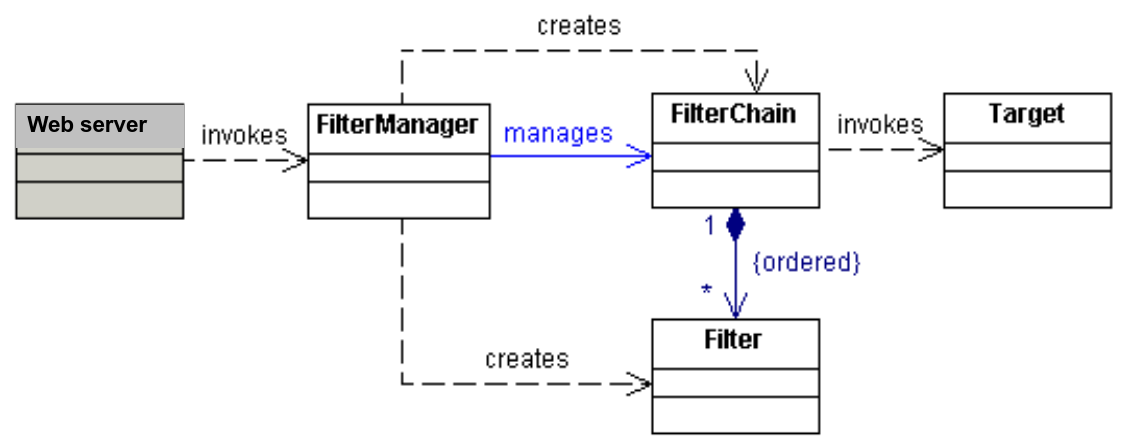
\includegraphics[width=1\linewidth]{images/intercepting_filter.png}
    \caption{Relazioni tra classi software in Intercepting Filter}
    \label{fig:intercepting_filter}
\end{figure}
Viene definito un Filter per ognuna delle funzionalità di Filtering. Ogni Filter è composto da una parte di pre-elaborazione e una di post-elaborazione. Non è però obbligatoria la presenza di entrambe: un filtro può infatti presentare solo una fase di pre-elaborazione o solo una fase di post-elaborazione.\\
\\
Una FilterChain raccoglie tutti i Filter che devono essere applicati a un certo tipo di richiesta: se viene ricevuta una richiesta che deve essere gestita con una particolare FilterChain, tutti le fasi di pre-elaborazione dei filtri presenti nella FilterChain vengono eseguite in ordine, per poi eseguire la logica di business corretta e infine eseguire tutte le post-elaborazioni, ma nell'ordine inverso rispetto all'ordine dei Filter all'interno della FilterChain.\\
\\
Un FilterManager raccoglie e gestisce tutte le possibili FilterChain, e si occupa di gestire una richiesta con la FilterChain corretta.
\begin{figure}[H]
    \centering
    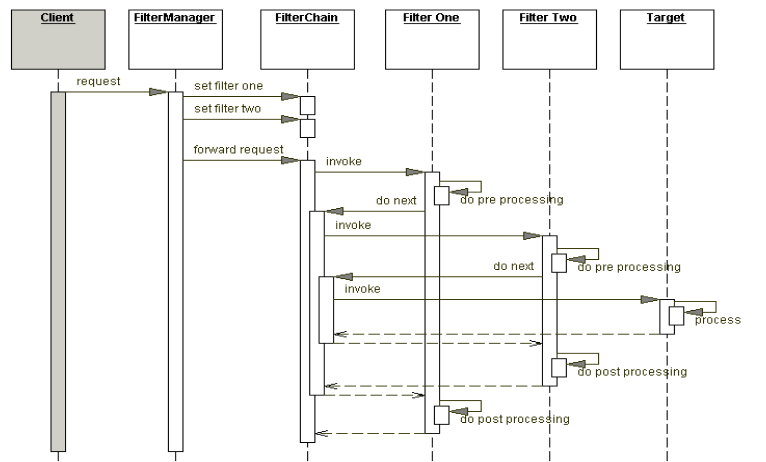
\includegraphics[width=1\linewidth]{images/filterchain_execution.png}
    \caption{Esempio di esecuzione dei filtri di una FilterChain}
    \label{fig:filterchain_execution}
\end{figure}


\subsection{View Design}
I View Design sono i pattern che è possibile seguire per implementare la View.

\subsubsection{Template View}
Il codice HTML di una pagina viene generato dinamicamente a partire da pagine template. Ogni pagina template è formata da una parte statica, ovvero codice HTML già specificato, e una parte dinamica, che genera altro codice HTML che andrà ad affiancarsi a quello già presente della parte statica.
La generazione della parte dinamica si basa sui dati contenuti nei modelli.
È solitamente usato congiuntamente a Page Controller.\\
\\
L'esecuzione della pagina dinamica può essere sia lato server che lato client: nel primo caso, il server genera completamente la pagina, e poi la invia al client; nel secondo caso, invece, il client riceve una pagina template, e procederà a eseguire richieste al Model lato server in modo da completare la pagina.

La scelta sul tipo di architettura (lato client o lato server) da adottare può basarsi sui seguenti criteri:
\begin{itemize}
    \item l'architettura lato server è più veloce nella costruzione della pagina completa se il numero di client è gestibile, altrimenti è consigliato gestire la costruzione della pagina lato client;
    \item l'architettura lato client permette di mostrare prima la pagina incompleta, ma richiede tempo per completarla;
    \item se i dati richiesti da una pagina cambiano spesso, allora è meglio utilizzare un'architettura lato client, in quanto permette di modificare solo piccole parti della pagina già presente sul client.
    L'architettura lato server richiederebbe infatti una rigenerazione dinamica dell'intera pagina, e il suo invio al client, a ogni modifica di un dato.
\end{itemize}

\subsubsection{Transform View}
In questo tipo di pattern, la View viene ottenuta tramite un processo di trasformazione: ogni dato di un Model viene infatti codificato in una stringa XML e una pagina viene generata combinando tutte le stringhe dei dati richiesti. Una pagina generata tramite Transform View è completamente dinamica: non sono infatti previste parti statiche.
\\
Quando una stringa XML viene richiesta, ovvero il relativo dato deve essere mostrato, essa viene passata a un classe Transformer, che raccoglie tutte le stringhe XML dei dati richiesti e genera la pagina.
La generazione della pagina da parte del Transformer può essere modificata usando regole di personalizzazione: a ogni dato possono essere associate più regole, che permettono di modificarne il rendering.
Le regole sono specificate con un apposito linguaggio di trasformazione.\\
\\
Un possibile svantaggio che presente questo approccio è che non è possibile visualizzare la pagina, nemmeno incompleta, prima che siano state elaborate tutte le regole e generata l'intera pagina completa.
Inoltre, essendo la pagina risultante dipendente dai dati da cui è costruita, il testing può complicarsi. Si semplifica invece il testing delle regole di trasformazione, in quanto semplici stringhe.

\subsubsection{Two-step View}
DA FINIRE

\subsection{Spring MVC}
DA FINIRE
\chapter{Design pattern per l'interazione con un database relazionale}
\section{Gateway}
Il Model è quella parte del codice che incapsula e gestisce lo stato dell'applicazione, ovvero i suoi dati.
Gli oggetti che compongono il Model sono però salvati in memoria principale, e quindi può essere utile renderli persistenti in memoria secondaria: entra quindi in gioco il database, in cui si andranno a salvare i dati che si vogliono rendere persistenti.
Una volta introdotto, però, viene a crearsi un mismatch, in quanto la rappresentazione usata dagli oggetti di un linguaggio orientati agli oggetti è differente da quella usata dal database (in quelli relazionali sono tabelle). Di conseguenza, è necessario un componente che si occupi della traduzione in entrambi i sensi, che prende il nome di gateway: oltre che occuparsi della traduzione, il gateway incapsula il database come una risorsa esterna.

Il gateway può essere implementato in due modi:
\begin{itemize}
    \item active record: la persistenza viene gestita dagli oggetti stessi del Model. Conterranno infatti metodi appositi per effettuare le operazioni CRUD sul database, e quindi il gateway è implicitamente definito nel Model.\\
    I principali metodi che possono comparire in un oggetto del Model per gestire la persistenza con il database sono:
    \begin{itemize}
        \item load;
        \item constructor;
        \item finder;
        \item writer;
        \item getter/setter.
    \end{itemize}
    Gestire la persistenza degli oggetti con gli oggetti stessi sporca, però, le classi che definiscono il Model.
    \item data mapper: la persistenza viene gestita da componenti separati dal Model.
    Per ogni oggetto modello del Model, viene implementato un componente Mapper, che sa come leggere e scrivere l'oggetto associato dal/sul database.

    Essendo separati dal Model, i mapper possono essere generati automaticamente dai framework utilizzati.
\end{itemize}

\section{Unit of Work}
Quando gli oggetti in memoria vengono modificati e i relativi cambiamenti vogliono essere resi persistenti, possono essere adottati due approcci:
\begin{itemize}
    \item a ogni modifica di un oggetto in memoria, il cambiamento viene scritto immediatamente sul database. Questo approccio è poco efficiente, in quanto porta a eseguire molte chiamate al database su dati di piccole dimensione e richiede una transazione attiva per tutta la durata dell'interazione \footnote{Per interazione formate da molte richieste, questo porta a bloccare molte risorse per un lungo periodo di tempo.};
    \item memorizzare tutti i cambiamenti che affliggono il database effettuati durante una business transaction (interazione) senza renderli immediatamente persistenti. Al termine della business transaction viene aperta una transazione, tutte le modifiche vengono rese persistenti sul database e infine si chiude la transazione.
\end{itemize}
La Unit of Work è un pattern comportamentale che permette di implementare il secondo approccio: la UoW memorizza infatti tutti i cambiamenti applicati a oggetti in memoria durante la business transaction e offre metodi per confermare (commit) o annullare (rollback) la business transaction. I  Il suo scopo è quello di raccogliere tutti le modifiche effettuate sugli oggetti in memoria durante una business transaction, e renderli persistenti sul database in un'unica mandata al termine della transazione.
Per fare ciò, la UoW incapsula i metodi per l'esecuzione di operazioni CRUD sul database.

Ogni sessione ha una relativa Unit of Work, che memorizza le modifiche effettuate in quella sezione.

I principali compiti svolti dalla Unit of Work sono:
\begin{itemize}
    \item incapsulare le operazioni ACID sul database;
    \item mantenere l'integrità del database. Una Unit of Work infatti, se possibile, effettua tutta la transizione, e non solo parti di essa;
    \item gestisce risorse utilizzate in maniera concorrente, permettendo di evitare deadlock.
\end{itemize}

I metodi offerti da UoW sono:
\begin{itemize}
    \item commit: rende persistenti tutti i cambiamenti effettuati durante la business interaction.
    \item rollback: al verificarsi di qualsiasi errore (come una discrepanza tra numeri di versione) o se desiderato dall'utente, permette di annullare tutti i cambiamenti effettuati durante la business interaction.
\end{itemize}

\subsubsection{Locking delle risorse nel database}
Quando la UoW deve rendere persistenti le modifiche, deve essere possibile applicare qualche tipo di lock alle risorse nel database che si vogliono manipolare., in modo tale da mantenere la consistenza del DB.
Esistono quindi due approcci al problema:
\begin{itemize}
    \item optimistic locking: utilizzato quando la probabilità di generare un conflitto \footnote{Un conflitto si verifica quando diverse transazioni di diverse UoW operano sulla stessa risorsa del DB.} è bassa. Viene implementato associando un version number a ogni risorsa \footnote{Una risorsa è una qualsiasi entry di una tabella.}, che verrà incrementato a ogni modifica della risorsa stessa.
    Se un'operazione di scrittura su una risorsa dipende da valori letti da una risorsa (che può anche essere diversa) con un certo version number, allora prima di compiere la scrittura si dovrà controllare che il version number della risorsa di lettura abbia mantenuto il valore iniziale, e che quindi la risorsa associata non sia stata modificata. Se il version number è stato modificato, allora la transazione corrente viene annullata, facendone il rollback.
    \item pessimistic locking: utlizzato quando la probabilità di generare un conflitto è alta. Una UoW che deve apportare una modifica a una risorsa acquisisce un lock su quella risorsa per tutto il tempo necessario al completamento della transazione. Eventuali altre UoW che vorranno accedervi non potranno farlo. Questo approccio, però, riduce la concorrenza.
\end{itemize}

\subsubsection{Policy di notifica dei cambiamenti}
Quando un oggetto in memoria viene modificato, la UoW associata alla sessione memorizza il cambiamento. Per farlo, però, essa deve essere a conoscenza dell'avvenuta modifica.
Esistono quindi due approcci di notifica di una modifica alla UoW:
\begin{itemize}
    \item caller registration: è colui che ha modificato l'oggetto in memoria che si deve occupare di notificare la UoW. Permette di scegliere quali cambiamenti devono essere resi persistenti, ma proprio per questo aumenta il rischio di errori causati da mancate notifiche alla UoW.\\
    Dovendo essere accessibile solo dall'utente, la UoW è locale alla sola sessione dell'utente.
    \item object registration: è l'oggetto modificato che si deve occupare di notificare la UoW.
    Proprio per questo motivo, la UoW deve essere accessibile globalmente, in quanto ogni oggetto deve poter comunicare con essa. Con questo tipo di approccio, tutti i cambiamenti vengono automaticamente resi persistenti.
\end{itemize}

\section{Identity Map e Identity Field}
Quando dei dati contenuti nel DB vengono caricati in memoria, è possibile che vengano effettuate più operazioni di caricamento sulla stessa risorsa. Un approccio ingenuo prevederebbe quindi di caricare in memoria un numero di copie dell'oggetto pari al numero di operazioni di caricamento. Si può però facilmente intuire che questo approccio non è affatto efficiente, oltre che non garantire la consistenza dell'oggetto caricato in memoria \footnote{Usando più copie, una modifica a una copia non si ripercuote su tutte le altre. In questo caso la risorsa non è più consistente, in quanto sono presenti in memoria più oggetti che la rappresentano che contengono informazioni contrastanti.}

Viene quindi utilizzato il pattern Identity Map, che prevede di definire un oggetto che tiene traccia di quali risorse sono già presenti in memoria, evitando quindi la presenza di copie multiple.\\
Quando la logica di business necessita di caricare una risorsa dal DB, essa contatta il Finder, specificando l'ID univoco della risorsa che si vuole caricare. A sua volta, il Finder contatta la Identity Map, per verificare se la risorsa con quell'ID è già presente in memoria. Se la risorsa non è presente, allora l'Identity Map comunica al Finder che essa è da caricare. Altrimenti, essa ritorna la reference all'oggetto già caricato.

A ogni sessione è associata una differente Identity Map, che gestisce tutte le risorse associate a quella sessione.

Quando una risorsa viene caricata in memoria, sottoforma di oggetto, si manifesta un mismatch di identità: la risorsa nel database è infatti identificata univocamente tramite una primary key, mentre l'oggetto in memoria lo è da una reference.
Se quindi si volessero rendere persistenti le modifiche apportate a un oggetto, un eventuale framework non saprebbe a quale risorsa l'oggetto fa riferimento.\\
Per risolvere questo problema, ogni oggetto contiene un Identity Field, che solitamente corrisponde alla primary key della risorsa a cui fa riferimento.

\section{JPA}
JPA è un standard Java per l'Object Relational Model. Essendo uno standard, le diverse implementazioni \footnote{Alcuni esempi di framework Java per l'ORM sono Toplink e Hibernate.} possono differire tra loro, ma rispettano comunque tutte le regole imposte dallo standard stesso.

JPA offre tutti i pattern precedentemente visti, ma per farlo deve poter mappare correttamente gli oggetti in memoria su risorse del database, e viceversa. Questo compito è affidato al programmatore, che definirà il mapping usando particolari "suggerimenti" detti \textbf{annotazioni}.

\subsection*{Entity Classes e Entity Manager}
Una risorsa del database che viene caricata in memoria  viene rappresentata come un oggetto di una semplice classe Java con soli attributi e metodi getter e setter \footnote{Una classe di questo tipo è l'equivalente Java di una Plain Old Data struct di C++, con l'unica differenza che gli attributi sono privati e bisogna accedervi solo con metodi getter e setter.}. 
La logica di business si occupa di modificare questi oggetti quando vuole apportare modifiche a risorse sul database.

Quando la logica di business vuole rendere persistenti le modifiche effettuati agli oggetti in memoria, allora essa contatta una Entity Manager.

La Entity Manager è la classe che effettivamente implementa tutti i pattern del modello ORM precedentemente visti: mantiene quindi una Unit of Work, per tenere traccia dei cambiamenti, e gestisce un'Identity Map, per evitare di duplicare un oggetto in memoria.
A ogni sessione è associata un'Entity Manager diversa.

\begin{figure}[h]
    \centering
    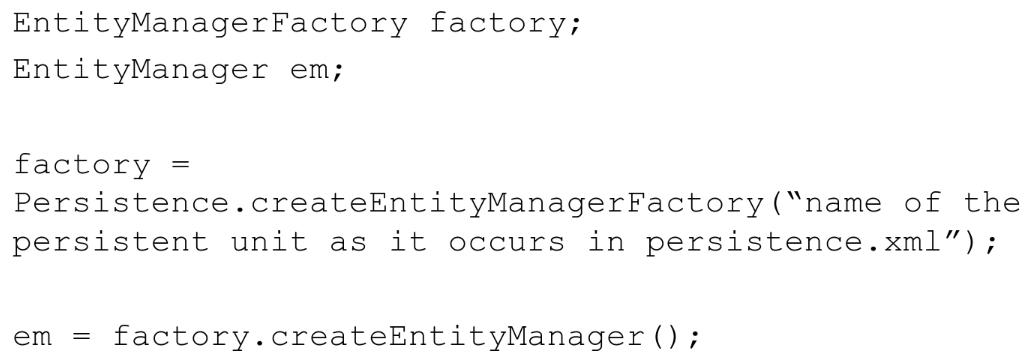
\includegraphics[width=1\linewidth]{images/entity_manager_factory.png}
    \caption{Creazione di un'Entity Manager tramite una Entity Manager Factory.}
    \label{fig:ent_man_factory}
\end{figure}

Per poter tenere traccia dei cambiamenti, però, essa deve poter essere a conoscenza sia della presenza in memoria degli oggetti che di eventuali cambiamenti apportati ad essi: bisogna quindi capire se il tipo di policy di notifica della UoW adottato è Caller Registration o Object Registration.\\
Nel caso di JPA, la creazione o distruzione di un oggetto deve essere segnalata dalla logica di business (Caller Registration), mentre i cambiamenti effettuati agli oggetti sono rilevati automaticamente (Object Registration).

I cambiamenti vengono però rilevati automaticamente solo se gli oggetti sono effettivamente monitorati dalla Entity Manager, ovvero la logica di business si è occupata di segnalare la loro presenza in memoria.
Un oggetto di una Entity Class può quindi trovarsi in due stati:
\begin{itemize}
    \item managed: la logica di business ha comunicato il caricamento in memoria dell'oggetto all'Entity Manager, e l'oggetto è quindi monitorato.
    \item unmanaged: l'Entity Manager non è a conoscenza dell'oggetto. Possono quindi essere presenti in memoria più copie dello stesso oggetto \footnote{La copia monitorata dall'Entity Manager e una o più copie non monitorate.}, portando a inconsistenza e impossibilità nel rendere persistenti i cambiamenti.\\
    Questo caso si verifica principalmente nei sistemi distribuiti, quando la macchina riceve un oggetto dalla rete.
\end{itemize}

\subsubsection{Operazioni offerte da una Entity Manager}
Le principali operazioni offerte da una Entity Manager sono:
\begin{itemize}
    \item \verb|persist|: rende persistenti le modifiche apportate agli oggetti managed. In realtà, le modifiche non vengono immediatamente rese persistenti, ma solo schedulate.
    \item \verb|flush|: rende immediatamenti persistenti le modifiche apportate agli oggetti managed.
    \item \verb|find|: dato l'ID di una risorsa nel database, restituisce una reference al relativo oggetto in memoria. Se l'oggetto non è presente, allora lo carica completamente, ovvero tutti i campi sono inizializzati correttamente. L'oggetto caricato sarà in uno stato managed, ovvero monitorato dalla Entity Manager;
    \item \verb|getReference|: identico all'operazione di \verb|find|, ma l'oggetto viene caricato in maniera lazy;
    \item \verb|merge|: dato un oggetto non ancora monitorato dalla Entity Manager, permette di rendere l'oggetto managed. Se è già presente un oggetto managed con lo stesso ID di quello specificato, allora l'oggetto monitorato assumerà i valori di quello ricevuto in input dalla \verb|merge|;
    \item \verb|remove|: dato un oggetto managed, rende l'oggetto unmanaged e schedula la sua rimozione dalla memoria.
    \item \verb|refresh|: dato un oggetto, cancella tutte le modifiche apportate a quell'oggetto e non ancora rese persistenti. Per farlo, ricarica dal DB la risorsa con l'ID specificato.
\end{itemize}

\subsection*{Mapping e annotazioni}
Gli oggetti in memoria e le risorse nel database devono mantenere un mapping consistente. Per farlo, JPA offre le annotazioni, particolari "suggerimenti" specificati dal programmatore nelle Entity Class che permettono alla Entity Manager di capire come un oggetto si traduce nel database.

Le annotazioni sono molte. Le più importanti sono:
\begin{itemize}
    \item \verb|@Entity|: posto prima della signature di una Entity Class, specifica che l'oggetto è mappato in una tabella del DB con lo stesso nome e la stessa struttura della Entity Class.
    \item \verb|@Table(name="...")|: posto prima della signatured di una Entity Class, specifica che l'oggetto è mappato in una tabella del DB di nome \verb|...| e con la stessa struttura dell'oggetto.
    \item \verb|@Id|: posto prima del campo della Entity Class che identifica l'Identity Field.
    \item \verb|@Column(name="...")|: posto prima di un campo della Entity Class, specifica che il campo è mappato in una colonna di nome \verb|...| nella tabella associata alla Entity Class.
    \item \verb|@SecondaryTable(name="...", @pkJoinColumns(@PrimaryKeyJoinColumn(name="...")))|: l'oggetto è mappato in due tabelle del DB, il cui nome della prima è quello della Entity Class, il nome della seconda è invece quello specificato nell'annotazione. L'oggetto corrisponde quindi a una join delle due tabelle.
\end{itemize}

\subsubsection{Mappare la cardinalità delle relazioni}
Le Entity Class possono essere in relazione tra loro, e ognuna di queste relazioni può avere una sua cardinalità.
I quattro tipi di relazioni sono:
\begin{itemize}
    \item uno-a-uno. In questo tipo di relazione, un'Entity Class possiede un campo contenente un singolo oggetto dell'altra Entity Class.
    Nel database, le due entità sono invece memorizzate in due tabelle diverse, e sarà necessaria nell'entità principale una foreign key alla primary key dell'entità secondaria.\\
    L'Entity Manager rileva questo tipo di relazione grazie a due annotazioni:
    \begin{itemize}
        \item \verb|@OneToOne|
        \item \verb|@PrimaryKeyJoinColumn|: specifica che il campo dell'entità principale si traduce in una foreign key alla primary key dell'entità secondaria.
    \end{itemize}
    \item molti-a-uno. FINIRE
    \item uno-a-molti. In questo tipo di relazione, un'Entity Class possiede una collezione di oggetti di un'altra Entity Class.
    Nel database, la tabella associata all'Entity Class secondaria contiene tutti i record contenuti nelle collezione. Ogni record contiene però anche una foreign key alla primary key del record nella tabella associata all'Entity Class principale che rappresenta l'entità che possiede la collezione.
    \item molti-a-molti. FINIRE
\end{itemize}
\chapter{Metodi agili e DevOps}
I metodi agili sono tutti quei metodi di sviluppo che:
\begin{itemize}
    \item gestire meglio i cambiamenti di requisiti;
    \item si concentrano sulle persone anziché sulla produzione di artefatti. In processi di sviluppo classici, infatti, la documentazione molto spesso viene prodotta per poi non essere utilizzata;
    \item prevedono una comunicazione diretta e verbale all'interno del team, e anche tra team e stakeholder;
    \item prevedono un testing continuo dell'applicazione, in modo da individuare il più presto possibile eventuali errori.
\end{itemize}

La struttura di un generico processo agile prevede la presenza di diverse iterazioni, ognuna dedicata a un sottoinsieme di requisiti.\\
A inizio progetto, il team procede con uno studio parziale dei requisiti richiesti dagli stakeholder.
Vengono poi eseguite le iterazioni, ognuna con una durata specifica. Prima di ogni iterazione, il team sceglie un sottoinsieme di requisiti su cui si vuole concentra nella successiva iterazione.
Alla fine di un'iterazione, il team avrà prodotto una parte del software completo ma già funzionante e possibilmente testata e integrata.
Idealmente, il team non dovrebbe tornare a lavorare su parti del prodotto finale sviluppate in precedenti iterazioni, a meno di cambiamenti nei requisiti.

Alcuni esempi di metodi agili sono Scrum e Extreme Programming (XP).

\section{Scrum}
Scrum è un processo agile con iterazioni di durata compresa tra 1 e 4 settimane.

\begin{defn}
    Uno \textbf{Sprint} è un'iterazione del processo Scrum.
\end{defn}

\begin{defn}
    Un \textbf{Daily Scrum meeting} è un incontro che si tiene ogni giorno (solitamente la mattina) a cui partecipano tutto il team e lo Scrum Master.

    Durante il Daily Scrum meeting, il team discute brevemente sullo stato dell'iterazione e su cosa fare durante la giornata.
\end{defn}

\begin{defn}
    Il \textbf{product backlog} è l'insieme dei requisiti parziali definito all'inizio del progetto.
\end{defn}

\begin{defn}
    Lo \textbf{Sprint backlog} è il sottoinsieme dei requisiti scelti per una determinata iterazione.
\end{defn}

\begin{defn}
    Lo \textbf{Spring planning meeting} è un incontro che si tiene all'inizio di ogni iterazione, in cui vengono definiti la durata dell'interazione e lo Sprint backlog.
\end{defn}

\begin{rem}
    Alla fine di ogni iterazione, il team effettua un altro iincontro, in cui discute di eventuali criticità rilevate durante l'iterazione.
\end{rem}

Il processo Scrum prevede i seguenti ruoli:
\begin{itemize}
    \item team: si occupa dello sviluppo del software;
    \item Scrum master: controlla che il processo Scrum sia correttamente applicato;
    \item product owner: rappresentante di tutti gli stakeholder, a conoscenza di tutti i requisiti che il software deve rispettare.
\end{itemize}

\section{DevOps}
Il processo di sviluppo di un software è distribuito tra tre entità: stakeholder, team di sviluppo e team di operations. Le relazioni tra queste entità sono stakeholder-team di sviluppo e team di sviluppo-team di operations \footnote{Il team di operations si occupa di mettere in campo e rendere operativo il sistema sviluppato dal team di sviluppo. Effettuano inoltre il monitoring del sistema.}.\\
I metodi agili permettono di migliorare la relazione tra stakeholder e team di sviluppo ma, in alcuni casi, può essere utile anche migliorare la relazione tra team di sviluppo e team di operations, soprattutto in casi di frequenti release che modificano il sistema.

DevOps permette quindi di semplificare e facilitare la messa in campo delle release prodotte dal team di sviluppo.

DevOps si basa su una forte \textbf{automazione} dei processi e sulla loro \textbf{ripetibilità}.
Tutti i processi automatizzati implementati da DevOps riguardano:
\begin{itemize}
    \item Continous Development: 
    \item Continous Integration: processi che si occupano di integrare correttamente i cambiamenti nel sistema esistente.
    \item Continous Testing: processi che si occupano di verificare l'adeguatezza dei cambiamenti apportati.
    \item Continous Deployment: processi che si occupano di rendere operativo il sistema a cui sono state apportate modifiche.
    \item Continous Monitoring: processi che si occupano di monitorare il sistema e ottenere feedback.
\end{itemize}

I feedback in DevOps, quindi, non sono raccolti dagli utenti, ma da tool automatici, che forniscono aggiornamenti continui e dettagliati sullo stato del sistema.

I ruoli previsti da DevOps sono:
\begin{itemize}
    \item DevOps Evangelist: colui che conosce la pratica DevOps e controlla che sia applicata. Nella pratica, l'evangelist non è quasi mai presente ma vengono adottati gli strumenti tipici di DevOps;
    \item automation expert: colui che gestisce i processi di automazione, creandoli e modificandoli quando necessario;
    \item release manager;
    \item figura per la Quality Assurance;
    \item ingegnere della sicurezza.
\end{itemize}

DevOps segue 6 principi: la cosa più importante è che tutto deve essere automatizzato, testato e monitorato.


\chapter{Git}
Git è un sistema di controllo di versione distribuito.

\section{Approcci allo sviluppo con Git}
Git può essere integrato in due modi all'interno di un processo di sviluppo software: GitFlow e Trunk-based.
\subsubsection{GitFlow}
Il GitFlow prevede la presenza di più branch all'interno del progetto Git. In particolare, le branch utilizzate sono:
\begin{itemize}
    \item main: branch principale che contiene il codice confermato e già rilasciato;
    \item development: branch secondario in cui risiede il codice modificato, ma ancora da rilasciare;
    \item hotfix: branch per situazione straordinarie, utilizzato per implementare modifiche urgenti al codice che risiede sul branch main. Nasce dal branch main, e al completamento del fix ne viene fatto il merge su main;
    \item feature \#n: branch dedicato all'implementazione della feature \#n. Nasce dal branch development e, al termine dell'implementazione della feature, ne viene fatto il merge sempre su development.
\end{itemize}

I vantaggi del GitFlow sono:
\begin{itemize}
    \item implementazione di processi di automazione dedicati per ogni branch. Un evento su una branch non esegue quindi processi automatizzati associati ad altre branch;
    \item ...
\end{itemize}

\subsubsection{Trunk-based}
Lo sviluppo Trunk-based con Git prevede l'esistenza di un unico branch main, che contiene il codice già rilasciato.\\
Quando uno sviluppatore vuole implementare una qualsiasi modifica, sia essa una nuova feature o una correzione al codice esistente, egli crea un branch di sviluppo dedicata di cui, al termine dell'implementazione, si farà la merge con il branch main.

Lo sviluppo Trunk-based è più rapido e facile da gestire, ma più rischioso, in quanto i cambiamenti finiscono direttamente nel branch principale. \upperAccE quindi adatto a progetti che coinvolgono solo sviluppatori esperti.

\section{DevOps}
Uno processo di sviluppo che usa Git può essere dotato di processi automatizzati per il DevOps: al verificarsi di particolari tipi di eventi nel repositiry Git, infatti, possono essere lanciati specifici processi con funzioni particolari.

I processi eseguiti a seguito dell'implementazione di una modifica formano un \textbf{Quality Gate}: la modifica è approvata solo se tutti i processi, che solitamente sono processi di test, terminano con successo.

Quando si implementa una modifica, i quality gate
Quality gate per piccole modifiche:
\begin{itemize}
    \item unit test;
    \item code review delle push request;
    \item analisi statica del codice.
\end{itemize}
Questo tipo di quality gate viene usato ad esempio, in un approccio GitFlow, a seguito di una merge di un ramo \verb|feature #n| e il ramo \verb|development|.

Quality gate per una parte del sistema che usa la piccola modifica:

\end{document}